\documentclass[conference]{IEEEtran}
\IEEEoverridecommandlockouts
% The preceding line is only needed to identify funding in the first footnote. If that is unneeded, please comment it out.
\usepackage[T1]{fontenc}
\usepackage{lmodern}
\usepackage{textcomp}
% Core Math & Theorems
\usepackage{amsmath,amssymb,amsfonts}
\usepackage{amsthm}
\usepackage{mathrsfs}
% Graphics & Floats
\usepackage{graphicx}
\usepackage{float}
\usepackage{placeins}
\usepackage{lscape}
% Tables
\usepackage{multicol}
\usepackage{array}
\usepackage{booktabs}
\usepackage{multirow}
\usepackage{makecell}
\usepackage{longtable}
\usepackage{threeparttable}
% Appendices & Links
% \usepackage[title]{appendix}
% \usepackage{url}
% Colors & Highlighting
\usepackage{xcolor}
\usepackage{soul}
\sethlcolor{cyan}
% \usepackage{hyperref}
\usepackage[colorlinks=true,linkcolor=blue,citecolor=blue,urlcolor=blue]{hyperref}
% Footnotes
\usepackage{manyfoot}
% Algorithms & Code
\usepackage{algorithm}
\usepackage{algorithmicx}
\usepackage{algpseudocode}
\usepackage{listings}

% Arabic packages
\usepackage{arabtex}
\usepackage{utf8}
\setcode{utf8}
% Patch for new LaTeX hook behavior (prevents "Loading a class or package in a group")
\makeatletter
\protected\def\begin#1{%
  \UseHook{env/#1/before}%
  \@ifundefined{#1}%
    {\def\reserved@a{\@latex@error{Environment #1 undefined}\@eha}}%
    {\def\reserved@a{\def\@currenvir{#1}%
        \edef\@currenvline{\on@line}%
        \@execute@begin@hook{#1}%
        \csname #1\endcsname}}%
  \@ignorefalse
  \begingroup
  \let\end\a@l@end
  \@endpefalse\reserved@a}
\makeatother
% % Theorem Environments
% \theoremstyle{thmstyleone}
% \newtheorem{theorem}{Theorem}
% \newtheorem{proposition}[theorem]{Proposition}
% \theoremstyle{thmstyletwo}
% \newtheorem{example}{Example}
% \newtheorem{remark}{Remark}
% \theoremstyle{thmstylethree}
% \newtheorem{definition}{Definition}
\usepackage[most]{tcolorbox}
\tcbuselibrary{breakable}
\newtcolorbox{mybox}{
  colback=black!5!white,
  colframe=black,
  arc=5pt,
  boxrule=0.8pt,
  width=\textwidth,
  before skip=10pt, % Add space before the box
  after skip=10pt   % Add space after the box
}

\def\BibTeX{{\rm B\kern-.05em{\sc i\kern-.025em b}\kern-.08em
    T\kern-.1667em\lower.7ex\hbox{E}\kern-.125emX}}
\begin{document}

\title{Fine-Tuning vs. Prompt Engineering for Ordinal Mental-Health Severity Classification}


\maketitle

\begin{abstract}
Most existing work on mental health text classification frames the problem as a simple binary decision, which overlooks the gradual nature of psychological distress. In this paper, we convert a publicly available binary mental health dataset of 27,977 user-generated texts into an ordinal severity classification task on a 1--10 scale. We first relabel the data using large language models guided by a detailed few-shot prompt, and we select the most reliable labeler through an agreement study against a strong reference model. Three candidate labelers---Gemini 3.1 Flash Lite, Mistral Small 4, and Qwen3-Next 80B---are evaluated against Kimi K2.6 using Quadratic Weighted Kappa, MAE, and SAD; Qwen shows the strongest alignment with the reference and is selected for the remaining experiments. We then fine-tune three transformer encoders (RoBERTa-base, DeBERTa-Large, and MentalBERT) on the ordinally labeled data, applying stratified splitting, sliding-window tokenization, class-weighted loss, and label smoothing to address class imbalance and long input texts. Finally, we compare fine-tuning against prompt engineering with instruction-tuned LLMs on the same held-out test set. Our results indicate that DeBERTa-Large achieves the best fine-tuning performance with an exact accuracy of 0.6372 and a QWK of 0.9504, while GPT-oss-20B leads the prompt-engineering approach with an exact accuracy of 0.4682 and a QWK of 0.9475. Overall, fine-tuned encoders substantially outperform prompt-based inference, suggesting that task-specific adaptation remains critical for fine-grained ordinal mental health classification.
\end{abstract}

\begin{IEEEkeywords}
Mental Illness, Fine-Tuning, Prompt Engineering, Encoders, LLMs
\end{IEEEkeywords}


%%%%%%%%%%%%%%%%%%%%%%%%%%%%%%%%%%%%%%%%%%%%%%%%%%%%%%%%%%%%%%%%%%%%%%%%%%%%%
\section{Introduction}
Mental-health conditions such as anxiety, depression, and suicidal ideation are among the most widespread health burdens worldwide, and a growing share of the people affected express their distress through user-generated text on social media and online forums. Most existing datasets and models, however, frame the problem as a binary decision, metally ill versus not not mentally ill which discards the degree of severity. In this work we transform a binary mental-health dataset \cite{mahawar2025genai} into an ordinal severity-classification task on a $1$--$10$ scale. We first relabel the data using LLMs guided by a prompt, and select the most reliable labeler through a proof-of-concept agreement study against a strong reference model. We then use this ordinally labeled dataset to find out when working on such a task, which approach is a better choice: fine-tuning a transformer encoders, or prompt engineering general-purpose LLMs? 

The main contributions of this paper are summarised as follows:
\begin{itemize}
    \item Converted a binary mental-health dataset into an ordinal 1--10 severity dataset through a defined prompt with few-shot examples LLM annotation.
    \item We fine-tune and benchmark three transformer encoders
    (RoBERTa-base, DeBERTa-Large, and MentalBERT) for ordinal severity
    classification, using imbalance and ordinal-aware techniques such as
    class-weighted loss and sliding-window tokenization.
    \item We provide a comparison of fine-tuning against prompt engineering with instruction-tuned LLMs, evaluated on the same test split
    with a common set of ordinal and bucket-level metrics.
\end{itemize}

%%%%%%%%%%%%%%%%%%%%%%%%%%%%%%%%%%%%%%%%%%%%%%%%%%%%%%%%%%%%%%%%%%%%%%%%%%%%%%%%
\section{Related Work}

Recent advancements in natural language processing have significantly improved mental health text analysis, particularly with the emergence of large language models (LLMs). Prior studies have explored multiple paradigms, including traditional machine learning pipelines, fine-tuned transformer models, and prompt-based LLM inference for mental health classification and severity estimation.

Kallstenius et al. \cite{Kallstenius2025} conducted a comprehensive evaluation comparing traditional NLP approaches with large language models for mental health status classification. Their study employed classical feature extraction techniques such as TF-IDF combined with machine learning classifiers, including Logistic Regression and Support Vector Machines, as well as transformer-based and instruction-tuned LLMs. All models were evaluated under a unified experimental setup to ensure fair comparison. The results demonstrated that transformer-based models consistently outperform traditional NLP methods in capturing contextual and semantic patterns in mental health text. However, the study is limited to binary and coarse-grained classification and does not explore ordinal severity modeling or fine-grained psychological state representation.

In a clinical context, Weber et al. \cite{Weber2025} proposed a fine-tuned large language model for symptom-based depression severity estimation using structured patient-reported datasets. Their approach mapped clinical symptom descriptions to severity levels aligned with standardized clinical assessment scales. The results showed strong agreement with expert annotations, demonstrating the effectiveness of fine-tuned LLMs in automated mental health assessment. However, the study is limited to clinical datasets and does not consider noisy real-world social media text or compare fine-tuning with prompt-based inference strategies.

More recently, Kermani et al. \cite{kermani-etal-2025-systematic} investigated different LLM adaptation strategies for mental health text analysis, including fine-tuning, prompt engineering, and retrieval-augmented generation (RAG). Their results indicate that fine-tuning generally achieves superior predictive performance, while prompt engineering provides a computationally efficient alternative with lower training and deployment cost. However, their work focuses on general classification tasks and does not evaluate ordinal severity modeling or encoder-based transformer architectures within a unified experimental framework.

Despite these advancements, existing studies still exhibit several limitations. First, most prior work formulates mental health analysis as a binary or coarse-grained classification task, which fails to capture gradual variations in psychological severity. Second, clinical studies are typically based on structured datasets that do not reflect the complexity and noise of real-world user-generated text. Third, limited work provides a controlled comparison between transformer encoder fine-tuning and prompt-engineered large language models under a unified ordinal severity setting.

These limitations indicate that the trade-off between different LLM adaptation strategies for fine-grained ordinal mental health modeling remains insufficiently explored. 


%%%%%%%%%%%%%%%%%%%%%%%%%%%%%%%%%%%%%%%%%%%%%%%%%%%%%%%%%%%%%%%%%%%%%%%%%%%%%%%%
\section{Methodology}
This section presents the framework implemented for transforming the binary mental-health dataset \cite{mahawar2025genai} into a detailed severity classification task. The proposed methodology consists of three main phases: severity labeling and proof-of-concept reference model selection, supervised fine-tuning of transformer-based classifiers, and prompt-engineering-based evaluation using different large language models. Figure \ref{fig:pipeline} provides an overview of the complete experimental pipeline.

\begin{figure}[ht]
    \centering
    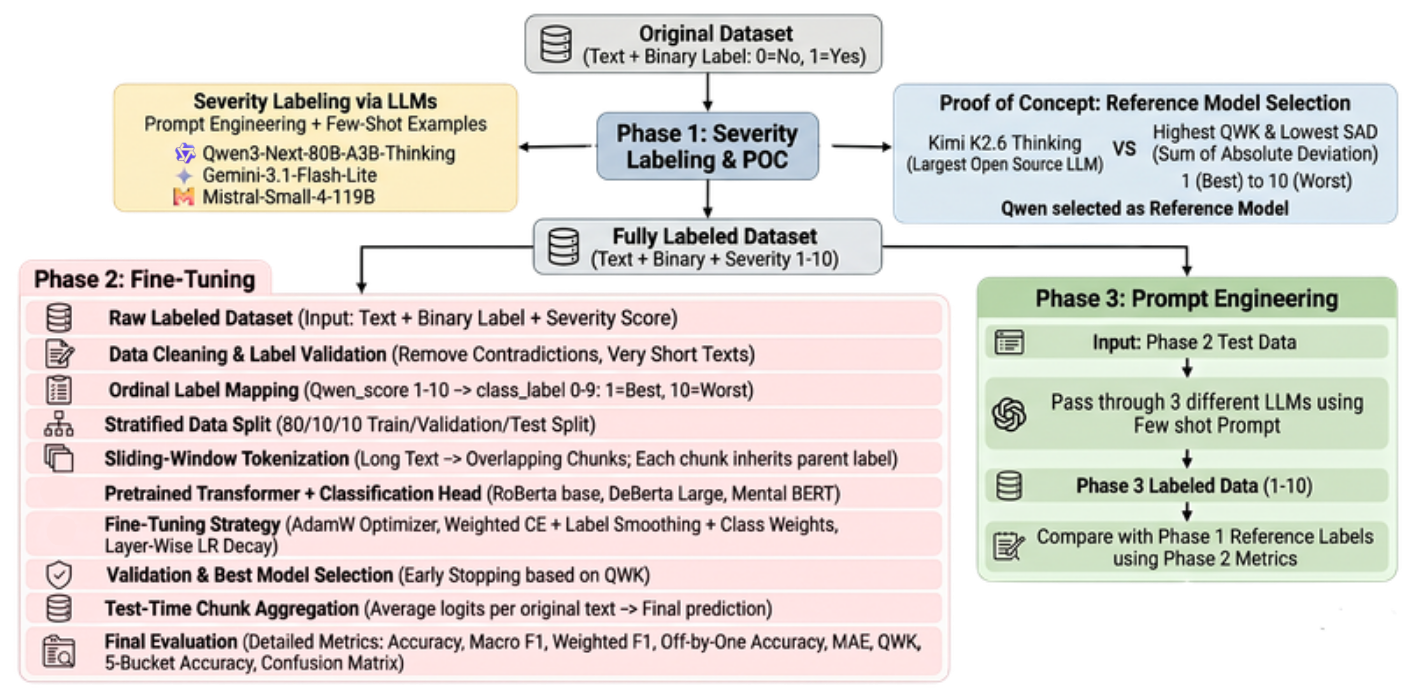
\includegraphics[width=\columnwidth]{pipeline.png}
    \caption{\centering Proposed Model Architecture}
    \label{fig:pipeline}
\end{figure}

\subsection{Dataset Description}
The Mental Health dataset \cite{mahawar2025genai} was used in our implementation. Each sample consists of user-generated text and a binary label that indicates the presence or absence of mental-health-related signals. The original data set contains two main fields: \textit{text} and \textit{label}. The \textit{text} column represents the textual content written by users, which may include expressions related to anxiety, depression, stress, suicidal ideation, emotional distress, or neutral everyday communication. The \textit{column} of labels is a binary indicator, where label 1 indicates that the text is associated with mental health issues or distress. In contrast, label 0 indicates that the text does not indicate mental health concerns. The dataset consists of 27,977 rows, of which 14,139 were labeled 0 (no mental illness) and 13,838 were labeled 1 (has mental illness).

Figure \ref{fig:dataset_sample} illustrates a sample of the dataset.

\begin{figure}[ht]
    \centering
    
\includegraphics[width=\columnwidth]{dataset_sample.png}
    \caption{\centering Dataset Sample}
    \label{fig:dataset_sample}
\end{figure}

\subsection{Dataset Processing \& Preparation}
Starting with the first phase, as shown in the pipeline Figure \ref{fig:pipeline}, the original dataset \cite{mahawar2025genai} provides only a binary label, which isn't enough for the detailed severity classification task. We therefore designed a three-stage relabeling and filtering pipeline that (i) converts each binary annotation into an ordinal severity score on a 1--10 scale, (ii) selects the labeling model to be used downstream through a proof-of-concept agreement study, and (iii) removes samples whose ordinal and binary labels are mutually inconsistent. The three stages are detailed below.

\subsubsection{Stage 1: Ordinal Severity Labeling with Multiple LLMs}
To enhance the binary annotations into ordinal severity scores, three large language models were used as separate labelers: Gemini 3.1 Flash Lite \cite{gemini31flashlite2026}, Mistral Small 4 119B \cite{mistralsmall4119b2026}, and Qwen3-Next 80B-A3B Thinking \cite{qwen3next80ba3bthinking2025}. Each model received a similar prompt shown in Figure \ref{prompt:mental_health_prompt}, together with a small set of few-shot examples, and assigned every sample a severity score from 1 to 10 according to the rubric defined in that prompt. This produced three sets of ordinal annotations for the dataset.

\subsubsection{Stage 2: Reference-Model Selection via a Proof-of-Concept Agreement Study} Because no ground-truth severity scores exist for the dataset, we specified a high-performing model to serve as a standard reference against which the three candidate labelers could be compared. We selected Kimi K2.6 Thinking \cite{kimiK2_2025} as the reference/verifier model. Kimi K2 \cite{kimiK2_2025} LLM is the highest-ranked open-weight model on the Artificial Analysis Intelligence Index \cite{artificialanalysis2026} and, with one trillion total parameters (32B active) in a Mixture-of-Experts (MoE) architecture, is among the largest openly available models. Adding to this, the K2 family achieves the strongest medical-domain performance among open-weight models: on the MLB clinical benchmark, it ranked first of ten leading models with 77.3\% overall accuracy \cite{mlb2026}, and it led the medical subdomain of the LPFQA professional-knowledge benchmark \cite{lpfqa2025}. Figure \ref{fig:kimi_benchmark} shows the performance of several open source best-performing models. The full dataset was relabeled with the reference model, and each candidate labeler (Gemini, Mistral, and Qwen) was then compared against the Kimi reference using three ordinal-agreement metrics: the Sum of Absolute Deviation (SAD) \cite{huber1964robust}, the Mean Absolute Error (MAE) \cite{willmott2005advantages}, and the Quadratic Weighted Kappa (QWK) \cite{articleQWK}. The 3 models that minimized SAD \cite{huber1964robust} and MAE \cite{willmott2005advantages} while maximizing QWK \cite{articleQWK} will be selected as the labeling model for the next fine-tuning and prompt-engineering phases. Qwen3-Next 80B-A3B Thinking \cite{qwen3next80ba3bthinking2025} achieved the lowest SAD and MAE and the highest QWK, indicating the closest alignment with the anchor model, and was therefore selected.

\subsubsection{Stage 3: Consistency Filtering}
Finally, a consistency check was applied to remove samples in which the assigned ordinal score contradicted the original binary label. Scores in the range $1$-$5$ correspond to no mental illness (binary label $0$) and scores $6$--$10$ correspond to mental illness (binary label $1$). Any sample whose ordinal score fell on the opposite side of this boundary from its binary label was treated as inconsistent and discarded. 

\begin{figure}[ht]
    \centering
    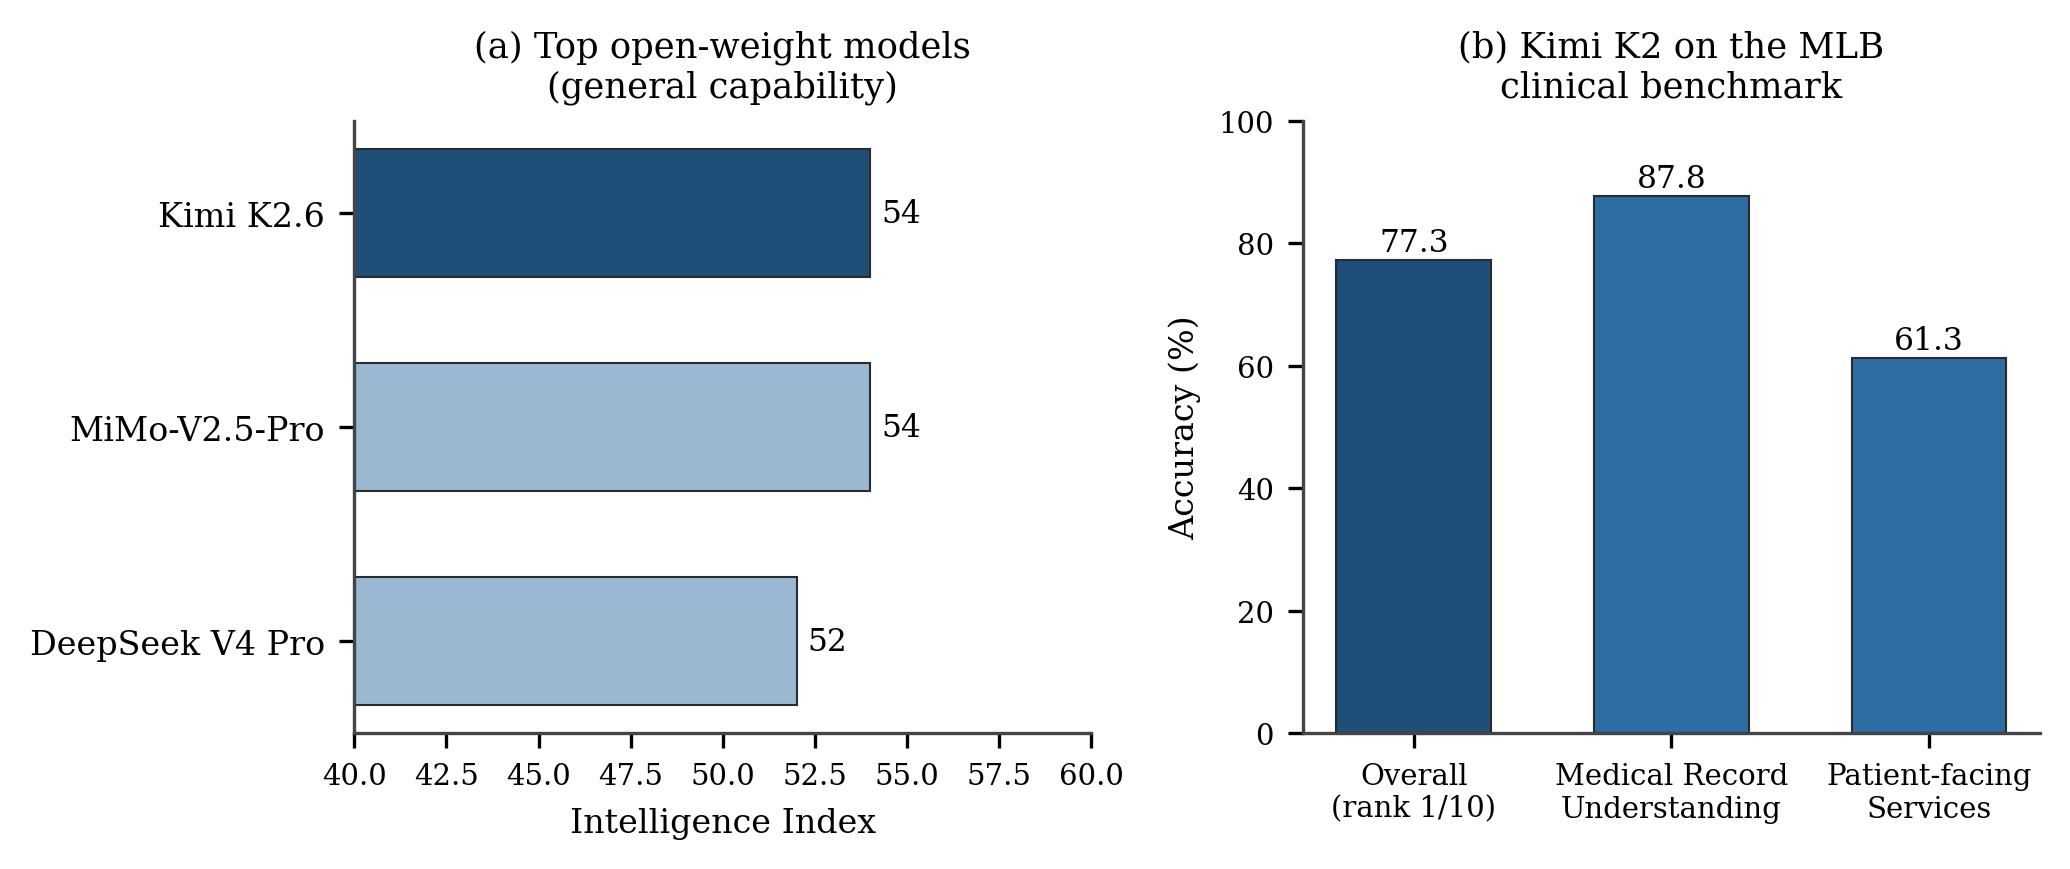
\includegraphics[width=\columnwidth]{kimi_benchmark.png}
    \caption{\centering 
    (a) Top open-weight models by general capability (Artificial Analysis Intelligence
    Index) \cite{artificialanalysis2026} (b) Kimi K2 performance on the MLB clinical
    benchmark, where it ranked first of ten evaluated models \cite{mlb2026}.}
    \label{fig:kimi_benchmark}
\end{figure}


\begin{figure*}[t]
\centering

\begin{tcolorbox}[
    enhanced,
    colback=black!5!white,
    colframe=black,
    title=Prompt,
    fonttitle=\bfseries,
    arc=4pt,
    boxrule=0.6pt,
    width=\linewidth,
    left=4pt,
    right=4pt,
    top=4pt,
    bottom=4pt,
    fontupper=\footnotesize
]
\begin{multicols}{2}

You are a clinical NLP expert and mental health classification assistant. Your task is to analyze a user's text message and determine the severity of their mental health condition on a scale from 1 to 10. The dataset contains user-generated comments related to anxiety, depression, stress, hopelessness, emotional distress, and suicidal ideation. Each sample includes a binary label:

\begin{itemize}
    \item \textbf{Label 0}: Mentally well ($\leq 5$)
    \item \textbf{Label 1}: Mentally distressed or at risk ($> 5$)
\end{itemize}

\vspace{2mm}
\textbf{Evaluation Criteria}
\begin{itemize}
    \item Emotional well-being and stability
    \item Anxiety, fear, or excessive worry
    \item Sadness, hopelessness, or emotional numbness
    \item Stress, burnout, or feeling overwhelmed
    \item Social withdrawal or isolation
    \item Suicidal ideation or self-harm references
\end{itemize}

\vspace{2mm}
\textbf{Rating Rubric}
\begin{itemize}
    \item \textbf{1 -- Excellent:} No signs of emotional distress or mental health concerns.
    \item \textbf{2 -- Very Good:} Mentally healthy with very minor emotional concerns.
    \item \textbf{3 -- Good:} Generally stable mental state with occasional mild stress or worry.
    \item \textbf{4 -- Mild Concern:} Slight emotional struggles or temporary stress, but functioning normally.
    \item \textbf{5 -- Neutral:} Emotionally mixed or borderline condition with unclear severity.
    \item \textbf{6 -- Moderate Distress:} Noticeable anxiety, sadness, stress, or emotional exhaustion.
    \item \textbf{7 -- Significant Distress:} Strong depressive symptoms, social withdrawal, or impaired functioning.
    \item \textbf{8 -- Severe Distress:} Intense hopelessness, emotional instability, or implicit suicidal thoughts.
    \item \textbf{9 -- Critical Condition:} Explicit suicidal ideation or severe psychological crisis requiring immediate attention.
    \item \textbf{10 -- Extreme Crisis:} Active suicidal risk, prior suicide attempts, or life-threatening mental condition.
\end{itemize}

\vspace{2mm}
\textbf{Instructions}
\begin{enumerate}
    \item Carefully analyze the user's text.
    \item Identify important linguistic and emotional indicators.
    \item Assign a severity score consistent with the label.
    \item Provide concise reasoning for the assigned score.
\end{enumerate}

\end{multicols}
\end{tcolorbox}

\caption{Prompt used for mental health severity scoring and classification}
\label{prompt:mental_health_prompt}

\end{figure*}

Figure \ref{fig:Class_Distribution} shows the ordinal labeling class distribution. 

\begin{figure}[ht]
    \centering
    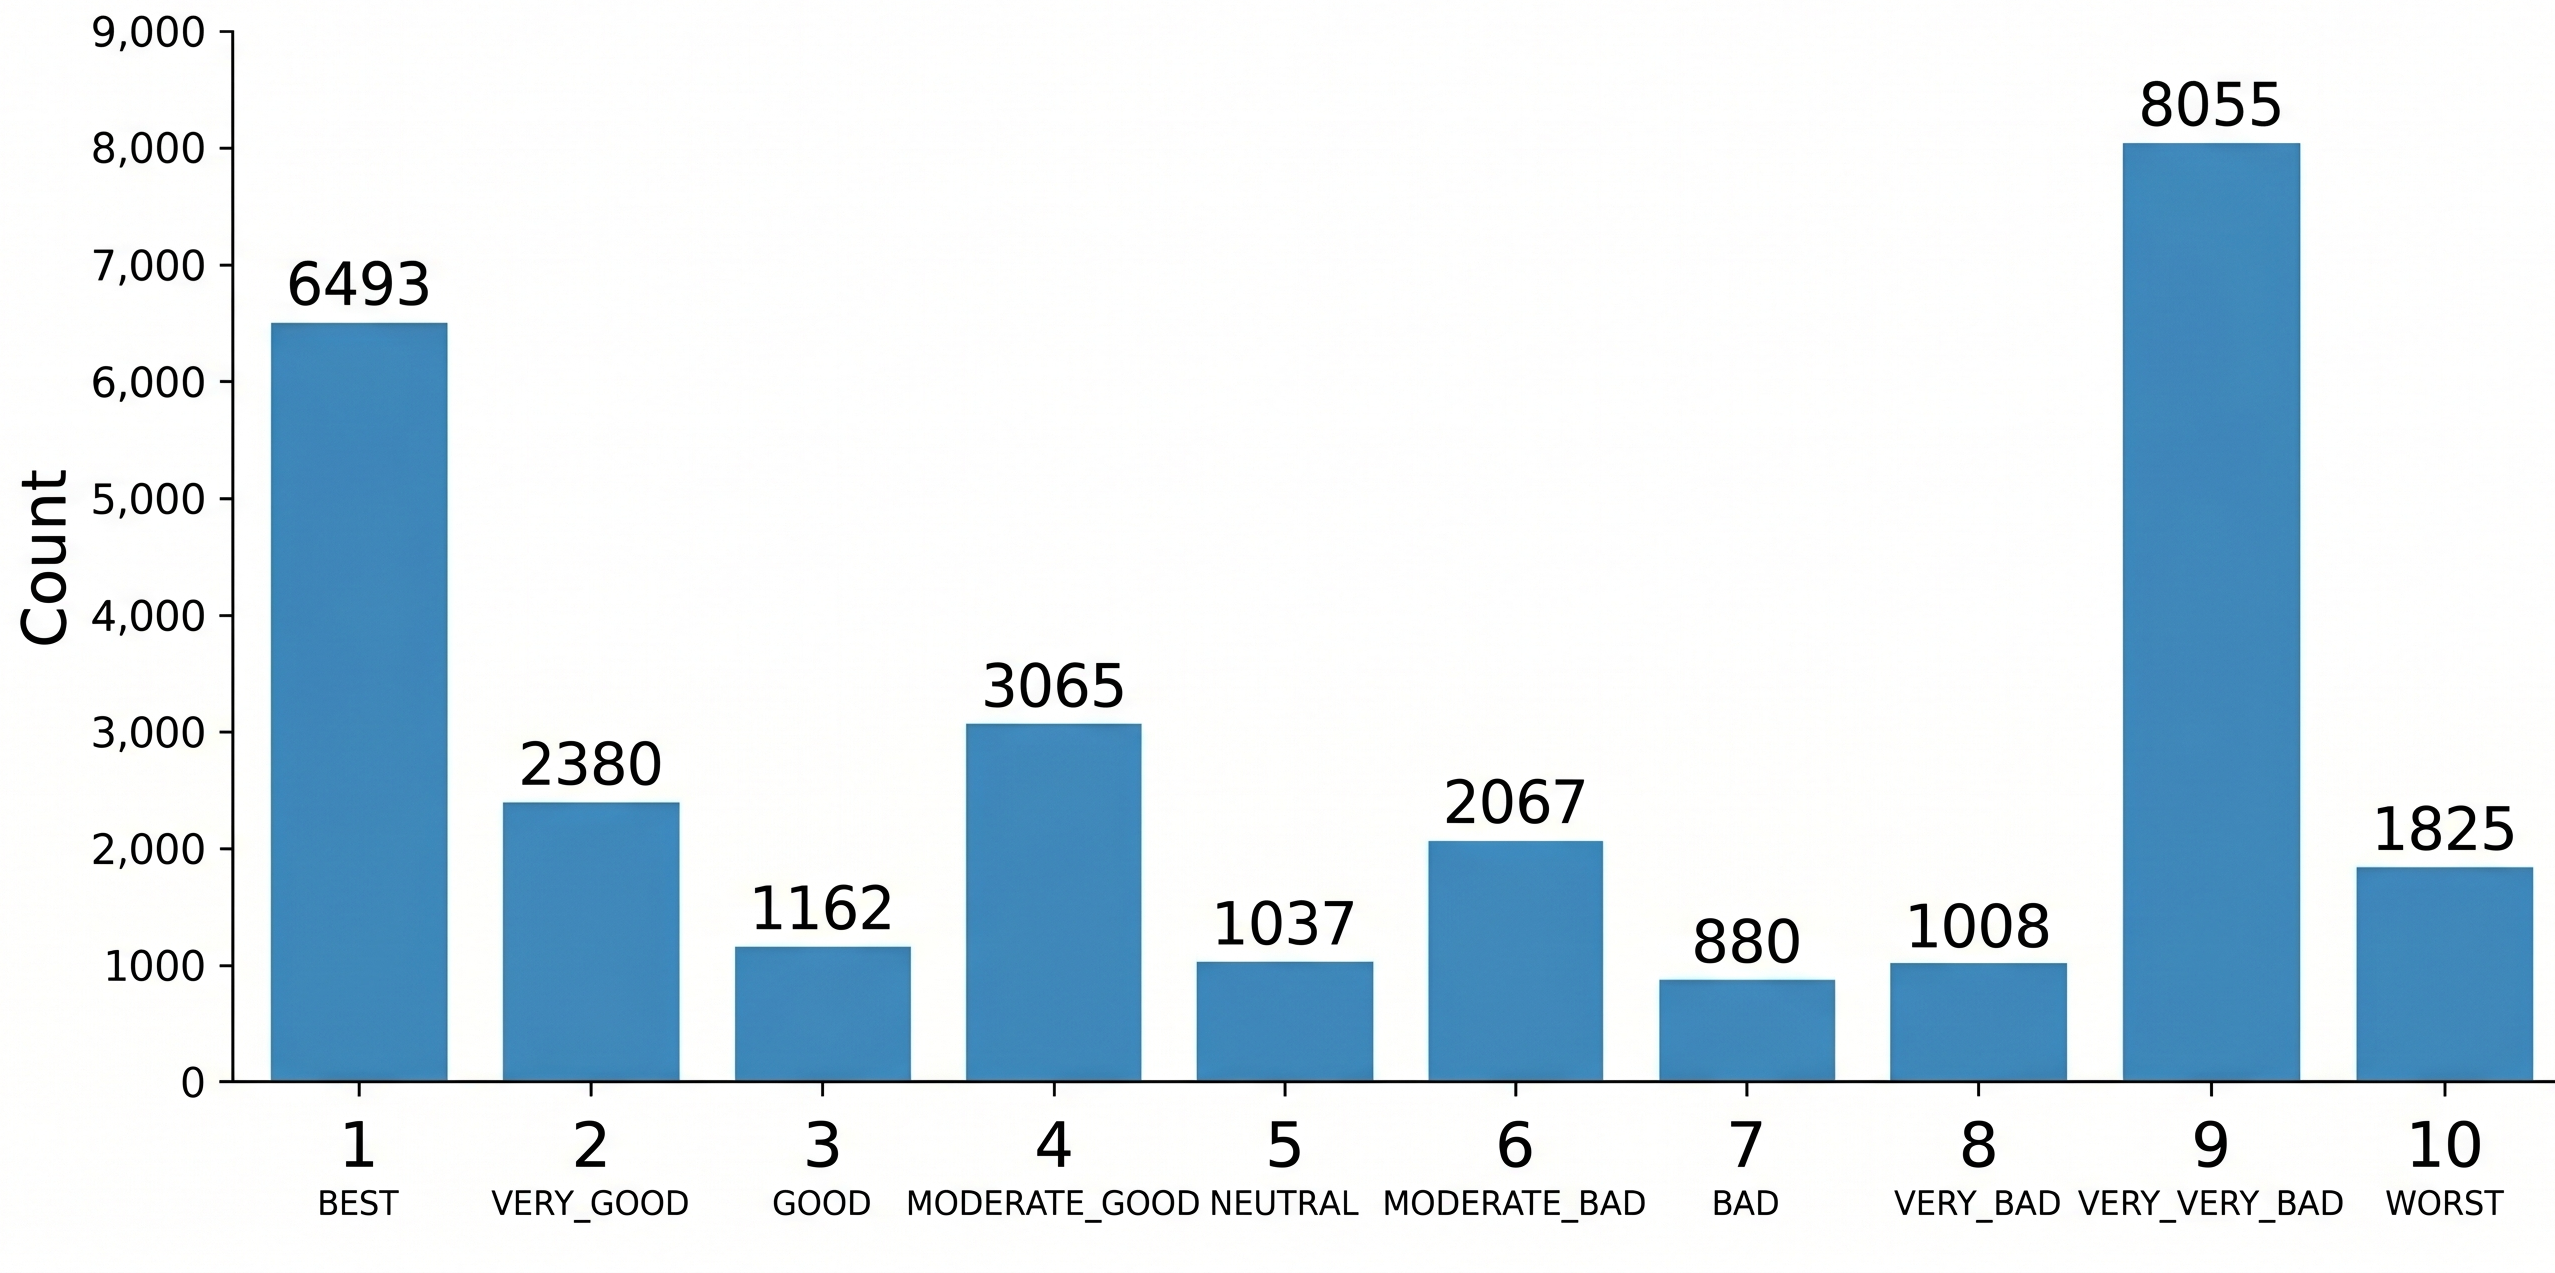
\includegraphics[width=\columnwidth]{Class_Distribution.png}
    \caption{\centering Ordinal Labeling Class Distribution}
    \label{fig:Class_Distribution}
\end{figure}
\subsection{Model Fine-Tuning}
Following the ordinal labeling of the dataset, we started with the fine-tuning
phase, in which we experimented with three pre-trained transformer encoders in
order to compare their performance on the task: RoBERTa-base
\cite{DBLP:journals/corr/abs-1907-11692}, DeBERTa-Large \cite{he2021deberta},
and MentalBERT \cite{ji2022mentalbert}.
To keep the comparison fair, an identical pre-processing pipeline was applied
before fine-tuning every encoder. First, because the class distribution is
highly imbalanced, the data were partitioned using stratified splitting, which
keeps the relative class proportions across the training, validation, and
test sets. Second, since all three encoders are limited to a maximum context
length of 512 tokens, we applied a sliding-window tokenization approach so that no information from longer inputs would be lost: instead of truncating, each long document was segmented into overlapping chunks (window size 512, stride 128), and every chunk inherited the label of its parent document. At inference time, the chunk-level predictions belonging to the same document were aggregated by averaging their logits, recovering a single prediction per text.


\subsubsection{\textbf{DeBERTa Large}}
DeBERTa Large \cite{he2021deberta} is a 24-layer transformer encoder with a
hidden size of 1024, 16 self-attention heads, and roughly 304M backbone
parameters. It improves on the BERT/RoBERTa family through two architectural
mechanisms: disentangled attention, in which each token is represented by
separate content and relative-position vectors, so that attention scores are
computed from both the contents and the relative distances of token pairs, and an enhanced mask decoder, which uses absolute position information when predicting masked tokens. Attaching a sequence classification head on top of the encoder: the contextual embedding of the leading [CLS] token is passed through a pooling dense layer and dropout, followed by a linear layer that projects onto the ten ordinal severity classes. A dropout probability of $0.2$ was applied to the hidden, attention, and head layers to regularize the comparatively large model. 
The encoder and head were fine-tuned for the ten-class ordinal classification task. To counter the class imbalance, we minimized a class-weighted cross-entropy loss in which each class contributes inversely to its frequency in the training set, and we combined it with a label-smoothing factor of $0.1$ to discourage over-confident predictions on the noisy, automatically generated labels. Optimization used AdamW (weight decay $0.05$, excluding bias and LayerNorm parameters) under a cosine learning-rate schedule with a $10\%$ warm up phase. We also used layer-wise learning-rate decay with a factor of $0.9$ and a base rate of $8\times10^{-6}$, so that layers closer to the input, which encode more general linguistic features, receive progressively smaller learning rates than the task-specific head; this keeps the pretrained knowledge while allowing the upper layers to adapt to the target domain. 


\subsubsection{\textbf{RoBERTa-Base}}
% \hl{Zeinab}
RoBERTa-Base \cite{DBLP:journals/corr/abs-1907-11692} is a transformer-based encoder consisting of 12 layers, a hidden size of 768, 12 self-attention heads, and approximately 125M parameters. It is an optimized variant of BERT that removes the Next Sentence Prediction objective and employs dynamic masking during pretraining, enabling richer contextual language representations. These modifications allow RoBERTa to capture semantic and syntactic relationships more effectively than the original BERT architecture.

For the ordinal mental health severity classification task, a sequence classification head was attached to the encoder, where the contextual representation of the classification token is passed through a dense layer to predict one of ten severity classes. Because some posts exceed the model’s maximum context length, a sliding-window tokenization strategy was employed using a maximum sequence length of 256 tokens and a stride of 128 tokens, allowing long texts to be processed through overlapping chunks while preserving contextual information.

A dropout probability of 0.2 was applied to the hidden and attention layers to improve regularization during fine-tuning. The model was trained for six epochs with a batch size of 16 using the AdamW optimizer under a cosine learning-rate schedule with a 10% warm-up phase. To mitigate class imbalance across severity levels, class-weighted cross-entropy loss was used, assigning weights inversely proportional to class frequencies. In addition, a label-smoothing factor of 0.1 was incorporated to reduce over-confident predictions on the automatically generated labels.

Optimization further employed layer-wise learning-rate decay with a factor of 0.9 and a base learning rate of $2\times10^{-5}$, enabling lower layers to preserve general linguistic knowledge while allowing upper layers and the classification head to adapt to the target domain. Early stopping with a patience of two evaluation rounds was used to prevent overfitting and select the best-performing checkpoint according to the Quadratic Weighted Kappa (QWK) metric.


\subsubsection{\textbf{MentalBERT}}
MentalBERT \cite{ji2022mentalbert} is a domain-specific encoder built on the RoBERTa-base architecture and further pre-trained on mental health-related text corpora. It keeps the same 12-layer, 768-hidden-size, 125M-parameter configuration as the standard RoBERTa-base but adds clinical vocabulary and representations tailored to psychological language. For this work we used the \texttt{mental-roberta-base} checkpoint from the same family.

Unlike the other two encoders, which were trained strictly as 10-class classifiers, we experimented with both classification and regression for this model. The classification setup used the same tokenization pipeline---maximum sequence length of 256 tokens with truncation---and the same training hyperparameters as RoBERTa-base: batch size 16, learning rate $2\times10^{-5}$, weight decay $0.01$, and early stopping with patience 2. To handle imbalance, we applied mean-based resampling rather than class-weighted loss, bringing every class to the average training frequency. After 5 epochs the model reached a QWK around $0.92$ and an off-by-one rate near $85\%$, but validation loss rose steadily after epoch 2, indicating clear overfitting.

We therefore added a regression head with a single output neuron and trained it with MSE loss on the continuous 1--10 scale, keeping all other settings unchanged. Validation MSE improved from $3.637$ to $2.758$ by epoch 3 and then plateaued; the trainer automatically restored this checkpoint. On the test set, the regression model achieved a mean absolute error of $0.845$, an exact-match accuracy of $39.8\%$, and an off-by-one accuracy of $85.1\%$. These results suggest that treating severity as a continuous spectrum can help this domain-specific encoder generalize better, though the exact accuracy stayed below the best classification runs from DeBERTa-Large and RoBERTa-base.



\subsection{Prompt Engineering}
In this phase, we reused the test split held out from the fine-tuning stage and passed each text row to several LLMs for labeling, using a single defined prompt \ref{prompt:mental_health_prompt} augmented with few-shot examples. Keeping the prompt identical across models isolates the effect of the underlying LLM and makes the resulting labels directly comparable. Three instruction-tuned LLMs were evaluated under this setup: GPT-oss-20b \cite{openai2025gptoss}, Gemma-3n-e4b-it \cite{google2025gemma3n}, and Llama-3.1-8B-Instruct \cite{meta2025llama31}.


\subsubsection{Gemma-3n-e4b-it}
Gemma-3n-e4b-it \cite{google2025gemma3n} is an open-weight, instruction-tuned
model. It is built on the MatFormer (Matryoshka Transformer) architecture, in which a smaller sub-model is nested inside a larger one so that only a subset of parameters needs to be activated for a given request; combined with Per Layer Embedding (PLE) caching and KV-cache sharing, this allows the model to operate with 4 billion effective parameters while substantially reducing its memory and compute footprint. The model is natively multi-modal, accepting text, image, and audio inputs, was trained across more than 140 languages, and supports a context window of 32K  tokens, which is more than sufficient to fit our prompt, few-shot examples, and each input text without truncation.

\subsubsection{GPT-oss-120B}
% \hl{Zeinab}
2. GPT-oss-20B: GPT-oss-20B \cite{openai2025gptoss} is an open-weight, instruction-tuned large language model developed by OpenAI. The model contains approximately 20 billion parameters and is optimized for instruction following, reasoning, and structured text generation tasks. GPT-oss-20B supports long-context processing, enabling it to handle lengthy prompts that include task instructions, evaluation criteria, and multiple few-shot examples within a single input. The model is designed to produce reliable and consistent outputs across a wide range of natural language processing tasks and supports structured response formats such as JSON, making it suitable for automated annotation and labeling pipelines. Its context capacity is sufficient to accommodate the complete prompt template and each input text without requiring truncation.


\subsubsection{Llama-3.1-8B-Instruct}
Llama-3.1-8B-Instruct \cite{meta2025llama31} is the smallest model in Meta's Llama 3.1 family, with 8 billion parameters and a 128K-token context window. It is instruction-tuned through supervised fine-tuning and reinforcement learning from human feedback, and handles multilingual text generation across a broad set of languages. Because of its compact size, it is considerably lighter than both GPT-oss-20B and the Gemma-3n checkpoint we tested.

We accessed the model through the NVIDIA API using the same few-shot prompt and rubric as the other two labelers. However, because an 8B parameter model is more prone to repetitive or collapsed outputs on long structured prompts, we relaxed the decoding parameters slightly: temperature was set to 0.2 and top-p to 0.7, with a maximum output length of 1024 tokens. This gives the model more room to generate varied CSV responses without drifting far from the rubric. On the test set, Llama achieved an exact accuracy of 0.4696, an off-by-one accuracy of 0.7881, a 5-bucket accuracy of 0.7312, a QWK of 0.9146, and a weighted F1 of 0.4624. Its exact accuracy narrowly surpassed GPT-oss-20B, and its 5-bucket accuracy was also the highest among the three prompt-engineered models. However, it fell behind on off-by-one accuracy and QWK, suggesting that while it occasionally lands on the right severity level, its overall ordinal consistency is not as strong as the larger models.
%%%%%%%%%%%%%%%%%%%%%%%%%%%%%%%%%%%%%%%%%%%%%%%%%%%%%%%%%%%%%%%%%%%%%%%%%%%%%
\section{Results \& Discussion}
This section presents the experimental setup used for our implementation, the evaluation metrics used to evaluate the models, and the experimental results achieved.

\subsection{Experimental Setup}
Our methodology consists of two different experiments: fine-tuning and prompt
engineering. All fine-tuning was performed on an T4 GPU. For both encoders, the number of output labels was set to 10 to represent the ordinal severity classes, and a stride of 128 tokens was used for the sliding-window tokenization. The two models differed only in their input length and learning rate: DeBERTa-Large used a maximum sequence length of 512 tokens and a learning rate of $8\times10^{-6}$, whereas RoBERTa base used a maximum sequence length of 256 tokens and a learning rate of $2\times10^{-5}$. All remaining hyperparameters were shared across both models. Specifically, they were trained with a batch size of $16$, a gradient accumulation step of 1, and a maximum of 6 epochs, and were regularized using a weight decay of 0.05, a warm-up ratio of 0.1, label smoothing of 0.1, layer-wise learning-rate decay of 0.9, and a dropout probability of 0.2. Optimization used AdamW together with a cosine learning-rate schedule, while early stopping with a patience of 2 epochs was applied. In every run, the best checkpoint was selected according to the Quadratic Weighted Kappa (QWK) on the validation set, which explicitly accounts for the ordinal nature of the severity labels.
For the second experiment, prompt engineering, the LLMs were accessed through the NVIDIA platform \cite{nvidia_build_2026}. Across all prompt-based implementations, decoding was kept deterministic by setting the temperature to 0 and \texttt{top\_p} to 0, with \texttt{max\_tokens} set to 4096.

\subsection{Evaluation Metrics}
We used a set of evaluation metrics chosen to suit the ordinal nature of the severity-labelling task, in which the labels lie on a graded 1--10 scale rather than forming unordered categories. The two experimental settings are assessed differently. Phase 1 (reference-model selection) measures how closely each candidate labeler agrees with the reference annotations, using the Sum of Absolute Deviation (SAD), the Mean Absolute Error (MAE), and the Quadratic Weighted Kappa (QWK). Phases 2 and 3 (fine-tuning and prompt engineering) measure severity-classification performance against the held-out labels, using the exact accuracy, the per-class and weighted F1-score, the off-by-one accuracy, the 5-bucket accuracy, and again the QWK.

In the definitions below, $N$ is the number of evaluated samples and $C{=}10$ the number of severity classes. For sample $i$, $y_i$ and $\hat{y}_i$ denote the true and predicted class indices (equivalently, the reference and candidate scores in Phase~1). For a class $c$, $\mathrm{TP}_c$, $\mathrm{FP}_c$, and $\mathrm{FN}_c$ are its true positives, false positives, and false negatives, $n_c$ is its support (number of samples), and its precision and recall are $P_c = \mathrm{TP}_c/(\mathrm{TP}_c+\mathrm{FP}_c)$ and $R_c = \mathrm{TP}_c/(\mathrm{TP}_c+\mathrm{FN}_c)$. 

\paragraph{Phase1: Agreement with the reference labeler}
\textbf{Sum of Absolute Deviation (SAD)} \cite{huber1964robust} accumulates, over the whole dataset, the absolute gap between each predicted score and its reference, expressed in class-index units. As the unnormalised $\ell_1$ distance, it grows with both how often and how badly the two disagree, giving a single dataset-level measure of total deviation for which lower is better.
\begin{equation}
\text{SAD} = \sum_{i=1}^{N}\big|\hat{y}_i - y_i\big|
\end{equation}

\textbf{Mean Absolute Error (MAE)} \cite{willmott2005advantages} is the per-sample average of that same absolute gap (so that $\text{SAD} = N\cdot\text{MAE}$). Unlike plain accuracy, it rewards near-misses in proportion to how close they are, which makes it a natural fit for ordinal labels where being off by one level is far preferable to being off by several; lower is better.
\begin{equation}
\text{MAE} = \frac{1}{N}\sum_{i=1}^{N}\big|\hat{y}_i - y_i\big|
\end{equation}

\textbf{Quadratic Weighted Kappa (QWK)} \cite{cohen1968weighted} measures the
agreement between predictions and labels after correcting for the agreement that would arise by chance, penalising each disagreement in proportion to the square of its distance on the ordinal scale. Confusing two distant severity levels is therefore punished far more heavily than confusing adjacent ones. It ranges from $1$ (perfect agreement) down to $0$ or below(chance-level or worse), so higher is better.
\begin{equation}
\kappa = 1 - \frac{\sum_{i,j} w_{ij}\,O_{ij}}{\sum_{i,j} w_{ij}\,E_{ij}},
\qquad w_{ij} = \frac{(i-j)^2}{(C-1)^2}
\end{equation}
where $O_{ij}$ is the observed number of samples with true class $i$ and predicted class $j$, and $E_{ij}$ is the count expected if the true and predicted labels were independent.

\paragraph{Phases 2 and 3: Severity-Classification Performance.}
\textbf{Exact accuracy} \cite{sokolova2009systematic} is the fraction of samples whose predicted class matches the true class exactly. It is the strictest of our metrics, awarding no credit for predictions that land on a neighbouring severity level, and therefore tends to understate performance on a fine-grained ordinal scale.
\begin{equation}
\text{Accuracy} = \frac{1}{N}\sum_{i=1}^{N}\mathbf{1}\big[\hat{y}_i = y_i\big]
\end{equation}

\textbf{Per-class F1-score} \cite{sokolova2009systematic} is, for a given severity class $c$, the harmonic mean of its precision and recall, balancing the two into a single value. Reporting it separately for every class exposes how well each individual level is recovered, revealing weaknesses on the rare, middle-of-the-scale classes that an aggregate score would otherwise mask.
\begin{equation}
\text{F1}_c = \frac{2\,P_c\,R_c}{P_c + R_c}
\end{equation}

\textbf{Weighted F1-score} \cite{sokolova2009systematic} summarises performance across all classes as a single number by averaging the per-class F1 with weights proportional to each class's support. This accounts for the strong class imbalance in our data: frequent classes contribute more, so the score reflects overall behaviour rather than being dominated by rare classes.
\begin{equation}
\text{F1}_{\text{weighted}} = \frac{1}{N}\sum_{c=1}^{C} n_c\,\text{F1}_c
\end{equation}

\textbf{Off-by-one accuracy} \cite{baccianella2009evaluation} relaxes exact accuracy by counting a prediction as correct whenever it falls within one class of the true label. It captures the practically relevant notion that adjacent severity levels are often interchangeable, so that a prediction one step away should not be treated as a full error.
\begin{equation}
\text{Off-by-one} = \frac{1}{N}\sum_{i=1}^{N}\mathbf{1}\big[\,|\hat{y}_i - y_i| \le 1\,\big]
\end{equation}

\textbf{5-bucket accuracy} \cite{sokolova2009systematic} is the exact accuracy computed after collapsing the ten fine-grained classes into five coarser severity bands, Healthy, Good, Neutral, Bad, and Critical, through a fixed mapping $B:\{1,\dots,C\}\!\rightarrow\!\{1,\dots,5\}$. It measures whether a prediction lands in the correct broad severity region, which is the level of granularity most relevant for triage even when the exact level is missed.
\begin{equation}
\text{5-bucket Acc} = \frac{1}{N}\sum_{i=1}^{N}\mathbf{1}\big[B(\hat{y}_i) = B(y_i)\big]
\end{equation}

\noindent The same per-class and weighted F1-scores defined above are also reported on these five collapsed buckets, and the QWK introduced in Phase 1 is reported here as well to quantify the ordinal closeness of the classifiers'predictions.


\subsection{Experimental Results}
This section will presents the achieved results throughtout the implemented experiements.

\subsubsection{Labeler Agreement with the Reference Model}
The consistency of the three LLM labelers (Qwen3-Next 80B-A3B Thinking, Mistral Small 4, and Gemini3.1 Flash Lite) and the Kimi K2.6 reference model is shown in Table \ref{tab:poc_agreement}, using the Sum of Absolute Deviation (SAD), the Mean Absolute Error (MAE), and the Quadratic Weighted Kappa (QWK).
\begin{table}[ht]
\centering
\caption{Agreement of the three candidate labelers with the Kimi K2.6 reference.}
\label{tab:poc_agreement}
\begin{tabular}{lccc}
\toprule
Model            & SAD~$\downarrow$ & MAE~$\downarrow$ & QWK~$\uparrow$ \\
\midrule
Qwen3-Next 80B   & \textbf{44013} & \textbf{1.5658} & \textbf{0.7954} \\
Mistral Small 4  & 46816          & 1.6655          & 0.7839 \\
Gemini 3.1 Flash & 45525          & 1.6196          & 0.7774 \\
\bottomrule
\end{tabular}
\end{table}

The three labelers all show ordinal agreement with the reference (QWK between $0.78$ and $0.80$), suggesting that the rubric-based prompt provides consistent severity scores across different LLMs. Qwen, however, is the strongest on all metrics, with the lowest SAD = 44,013 and MAE = 1.5658 and the highest QWK = 0.7954. It was therefore selected as the labeling model for the fine-tuning and prompt-engineering phases.

Figure \ref{fig:deviation_boxplot} shows the absolute deviation of each labeler per sample from the Kimi reference. From the boxplot we can see that Qwen has the tightest and most stable error distribution among the three, with a median absolute deviation of 1, an upper whisker of 5, and no extreme outliers, indicating that the worst-case disagreements with the reference are still bounded. Both Gemini (median 1) and Mistral (median 2) have heavier tails with outlying deviations up to 9 severity points. So not only does Qwen have the best aggregate scores, it also avoids the catastrophic, full-scale disagreements seen for the other two labelers.

\begin{figure}[ht]
    \centering
    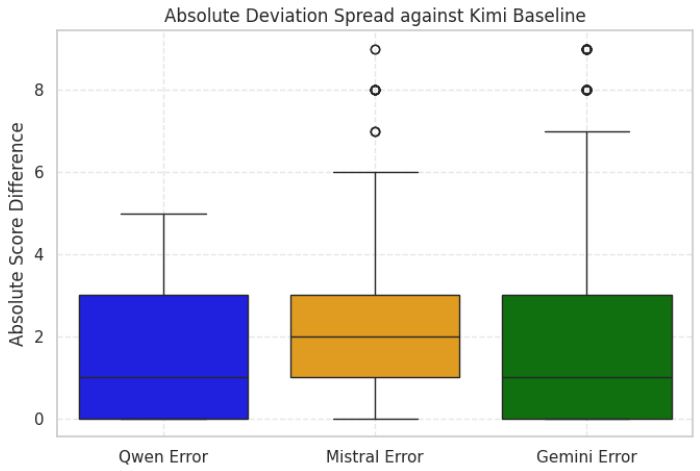
\includegraphics[width=\columnwidth]{deviation_boxplot.png}
    \caption{\centering Distribution of per-sample absolute score difference of
    each candidate labeler against the Kimi K2.6 baseline.}
    \label{fig:deviation_boxplot}
\end{figure}


\subsubsection{Fine-Tuning Results}
In this section, we report the performance obtained by the fine-tuned encoders on the test set (2,798). Table \ref{tab:ft_overall} summarizes the ordinal and bucket-level metrics. Table \ref{tab:ft_perclass_f1} provides the per-class F1-score on the full 10-class task and Table \ref{tab:ft_bucket_f1} shows the per-class F1-score after breaking down the predictions into the five varying severity buckets.

\begin{table}[ht]
\centering
\caption{Overall fine-tuning performance on the test set}
\label{tab:ft_overall}
\resizebox{\columnwidth}{!}{%
\begin{tabular}{lccc}
\toprule
Metric & RoBERTa-base & DeBERTa-Large & MentalBERT \\
\midrule
Exact accuracy (10-class) $\uparrow$ & 0.5443 & \textbf{0.6372} & -- \\
Off-by-one accuracy $\uparrow$       & 0.8581 & \textbf{0.8946} & -- \\
5-bucket accuracy $\uparrow$         & 0.7859 & \textbf{0.8306} & -- \\
QWK $\uparrow$                       & 0.9333 & \textbf{0.9504} & -- \\
F1 weighted $\uparrow$               & 0.5696 & \textbf{0.6545} & -- \\
\bottomrule
\end{tabular}}
\end{table}

\begin{table}[ht]
\centering
\caption{Per-class F1-score on the 10-class severity task.}
\label{tab:ft_perclass_f1}
\resizebox{\columnwidth}{!}{%
\begin{tabular}{lccc}
\toprule
Class & RoBERTa & DeBERTa & MentalBERT \\
\midrule
BEST            & 0.715          & \textbf{0.753} & -- \\
VERY\_GOOD      & 0.326          & \textbf{0.450} & -- \\
GOOD            & 0.282          & \textbf{0.349} & -- \\
MODERATE\_GOOD  & 0.531          & \textbf{0.638} & -- \\
NEUTRAL         & 0.418          & \textbf{0.434} & -- \\
MODERATE\_BAD   & 0.522          & \textbf{0.614} & -- \\
BAD             & \textbf{0.372} & 0.345          & -- \\
VERY\_BAD       & 0.272          & \textbf{0.356} & -- \\
VERY\_VERY\_BAD & 0.682          & \textbf{0.800} & -- \\
WORST           & 0.521          & \textbf{0.630} & -- \\
\midrule
Weighted avg    & 0.570          & \textbf{0.654} & -- \\
\bottomrule
\end{tabular}}
\end{table}

\begin{table}[ht]
\centering
\caption{Per-class F1-score on the collapsed 5-bucket task}
\label{tab:ft_bucket_f1}
\begin{tabular}{lccc}
\toprule
Bucket & RoBERTa & DeBERTa & MentalBERT \\
\midrule
Healthy  & 0.822 & \textbf{0.874} & -- \\
Good     & 0.630 & \textbf{0.720} & -- \\
Neutral  & 0.418 & \textbf{0.434} & -- \\
Bad      & 0.712 & \textbf{0.761} & -- \\
Critical & 0.920 & \textbf{0.920} & -- \\
\midrule
Weighted avg & 0.793 & \textbf{0.835} & -- \\
\bottomrule
\end{tabular}
\end{table}



\subsubsection{Prompt Engineering Results}
This section reports the performance of the prompt-based LLM labelers on the same held-out test set (2,798 documents) used for fine-tuning, for fair comparsion. Table \ref{tab:pe_overall} summarises the ordinal and bucket-level metrics, Table \ref{tab:pe_perclass_f1} gives the per-class F1-score on the full 10-class task, and Table \ref{tab:pe_bucket_f1} reports the per-class F1-score after collapsing the predictions into the five coarse severity buckets.

\begin{table}[ht]
\centering
\caption{Overall prompt-engineering performance on the test set}
\label{tab:pe_overall}
\resizebox{\columnwidth}{!}{%
\begin{tabular}{lcccc}
\toprule
Metric & Gemma-3n-e4b & GPT-oss & Llama-3.1-8B \\
\midrule
Exact accuracy (10-class) $\uparrow$ & 0.3989 & 0.4682 & \textbf{0.4696} \\
Off-by-one accuracy $\uparrow$       & 0.7402 & \textbf{0.8574} & 0.7881 \\
5-bucket accuracy $\uparrow$         & 0.6480 & 0.7198 & \textbf{0.7312} \\
QWK $\uparrow$                       & 0.9047 & \textbf{0.9475} & 0.9146 \\
F1 weighted $\uparrow$               & 0.4058 & \textbf{0.5091} & 0.4624 \\
\bottomrule
\end{tabular}}
\end{table}

\begin{table}[ht]
\centering
\caption{Per-class F1-score on the 10-class severity task}
\label{tab:pe_perclass_f1}
\resizebox{\columnwidth}{!}{%
\begin{tabular}{lcccc}
\toprule
Class & Gemma-3n-e4b & GPT-oss & Llama-3.1-8B \\
\midrule
BEST            & 0.349          & 0.669          & \textbf{0.695} \\
VERY\_GOOD      & 0.232          & 0.222          & \textbf{0.309} \\
GOOD            & 0.156          & \textbf{0.182} & 0.111 \\
MODERATE\_GOOD  & 0.318          & \textbf{0.485} & 0.280 \\
NEUTRAL         & 0.099          & \textbf{0.462} & 0.161 \\
MODERATE\_BAD   & 0.103          & \textbf{0.569} & 0.071 \\
BAD             & 0.161          & \textbf{0.276} & 0.020 \\
VERY\_BAD       & 0.181          & \textbf{0.200} & 0.126 \\
VERY\_VERY\_BAD & \textbf{0.747} & 0.587          & 0.716 \\
WORST           & 0.393          & \textbf{0.458} & 0.259 \\
\midrule
Weighted avg    & 0.406          & \textbf{0.509} & 0.462 \\
\bottomrule
\end{tabular}}
\end{table}

\begin{table}[ht]
\centering
\caption{Per-class F1-score on the collapsed 5-bucket task}
\label{tab:pe_bucket_f1}
\begin{tabular}{lcccc}
\toprule
Bucket & Gemma-3n-e4b & GPT-oss & Llama-3.1-8B \\
\midrule
Healthy  & 0.531          & 0.809          & \textbf{0.854} \\
Good     & 0.486          & \textbf{0.609} & 0.383 \\
Neutral  & 0.099          & \textbf{0.462} & 0.161 \\
Bad      & 0.600          & \textbf{0.660} & 0.513 \\
Critical & \textbf{0.886} & 0.762          & 0.850 \\
\midrule
Weighted avg & 0.644       & \textbf{0.728} & 0.725 \\
\bottomrule
\end{tabular}
\end{table}






%%%%%%%%%%%%%%%%%%%%%%%%%%%%%%%%%%%%%%%%%%%%%%%%%%%%%%%%%%%%%%%%%%%%%%%%%%%%%
\section{Conclusion}

This paper addressed the gap between binary mental health classification and fine-grained severity assessment by converting a 27,977-sample binary dataset into an ordinal 1--10 severity scale. Through a three-phase pipeline, we first relabeled the data using multiple LLMs with few-shot prompting and selected Qwen3-Next 80B as the most reliable labeler based on its agreement with a Kimi K2.6 reference. We then compared two approaches for severity classification: fine-tuning transformer encoders and prompt-engineering general-purpose LLMs.

Our results show that fine-tuned encoders substantially outperform prompt-based inference on this task. DeBERTa-Large achieved the strongest fine-tuning performance with an exact accuracy of 0.6372 and a QWK of 0.9504, while GPT-oss-20B led the prompt-engineering approach with a QWK of 0.9475 and a weighted F1 of 0.5091. The consistent gap between the two paradigms suggests that task-specific adaptation remains critical for fine-grained ordinal mental health classification, even when prompt engineering uses identical rubrics and few-shot examples. We also found that treating severity as a continuous regression target helped the domain-specific Mental-RoBERTa encoder generalize better than its classification counterpart, though it still underperformed the best classification runs.

A key limitation of this work is the absence of human clinical annotations; all severity scores were generated by LLMs, which introduces a risk of systematic bias. Future work could collect expert-rated labels, explore larger domain-specific encoders, and investigate ensemble methods that combine prompt-engineered labels with fine-tuned predictions.





%%%%%%%%%%%%%%%%%%%%%%%%%%%%%%%%%%%%%%%%%%%%%%%%%%%%%%%%%%%%%%%%%%%%%%%%%%%%%
\bibliographystyle{ieeetr}  
\bibliography{ref}

\end{document}
